\documentclass{beamer}

\usepackage[utf8]{inputenc}
\usepackage{clrscode3e}
\usepackage{gnuplot-lua-tikz}
\usepackage{tikz}

\usetikzlibrary{positioning}

\renewcommand{\gets}{\leftarrow}
\newcommand{\AND}{\land}
\newcommand{\IOR}{\lor}
\newcommand{\XOR}{\oplus}
\newcommand{\NOT}{\lnot}

\title{Using binary decision diagrams to determine program equivalence in a superoptimizer}
\author{Jesper Särnesjö}
\date{}

\begin{document}

\begin{frame}
\titlepage
\end{frame}

\begin{frame}
\end{frame}

\begin{frame}
\begin{figure}
\begin{tikzpicture}
\uncover<1->{\node (stc) [on grid]                   {stc};}
\uncover<2->{\node (i0)  [on grid,below=12mm of stc] {$i_0$};}
\uncover<2->{\path[->] (i0) edge (stc);}
\uncover<3->{\node (inc) [on grid,right=24mm of stc] {inc r0};}
\uncover<4->{\node (i1)  [on grid,below=12mm of inc] {$i_1 r$};}
\uncover<4->{\path[->] (i1) edge (inc);}
\uncover<5->{\node (add) [on grid,right=24mm of inc] {add r0,r1};}
\uncover<6->{\node (i2)  [on grid,below=12mm of add] {$i_2 r^2$};}
\uncover<6->{\path[->] (i2) edge (add);}
\uncover<7->{\node (pA)  [on grid,right=12mm of i0]  {$+$};}
\uncover<7->{\node (pB)  [on grid,right=12mm of i1]  {$+$};}
\uncover<7->{\node (eq)  [on grid,right=12mm of i2]  {$=$};}
\uncover<7->{\node (b)   [on grid,right=12mm of eq]  {$b$};}
\end{tikzpicture}
\end{figure}
\end{frame}

\begin{frame}[shrink]
\begin{figure}
\include{so_program_length_1}
\end{figure}
\end{frame}

\begin{frame}[shrink]
\begin{figure}
\include{so_program_length_2}
\end{figure}
\end{frame}

\begin{frame}[shrink]
\begin{figure}
\include{so_program_length_3}
\end{figure}
\end{frame}

\begin{frame}
\end{frame}

\begin{frame}
\begin{equation*}
\begin{array}{rcl}
\uncover<1->{s & \gets & a + b \\}
\uncover<2->{\langle s_1,s_0 \rangle & \gets & \langle a_1,a_0 \rangle + \langle b_1,b_0 \rangle \\}
\end{array}
\end{equation*}
\end{frame}

\begin{frame}
\begin{equation*}
\begin{array}{rcl}
\uncover<1->{s_0 & \gets & a_0 \XOR b_0 \\}
\uncover<2->{s_1 & \gets & a_1 \XOR b_1 \XOR a_0 \AND b_0 \\}
\end{array}
\end{equation*}
\end{frame}

\begin{frame}
\begin{equation*}
\begin{array}{rcl}
\uncover<1->{s_0 & \gets & a_0 \XOR b_0 \\}
\uncover<2->{c_0 & \gets & a_0 \AND b_0 \\}
\uncover<3->{s_1 & \gets & a_1 \XOR b_1 \XOR c_0 \\}
\uncover<4->{c_1 & \gets & a_1 \AND b_1 \IOR a_1 \AND c_0 \IOR b_1 \AND c_0 \\}
\end{array}
\end{equation*}
\end{frame}

%\begin{frame}
%$c_1 \gets (a_0 \AND a_1 \AND b_0) \IOR (a_0 \AND b_0 \AND b_1) \IOR (a_1 \AND b_1)$ % DNF
%
%$c_1 \gets (a_0 \IOR a_1) \AND (a_0 \IOR b_1) \AND (a_1 \IOR b_0) \AND (a_1 \IOR b_1) \AND (b_0 \IOR b_1)$ % CNF
%\end{frame}

\begin{frame}
\end{frame}

\begin{frame}
\begin{figure}
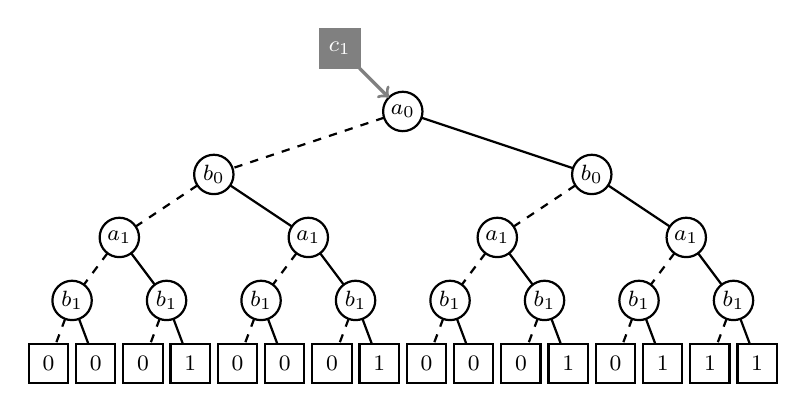
\begin{tikzpicture}
[every node/.style={draw=black,thick,minimum size=5mm,inner sep=0mm,outer sep=0mm,font=\footnotesize},
 var/.style={circle},
 val/.style={rectangle},
 ref/.style={rectangle,white,draw=gray,fill=gray},
 hl/.style={rectangle,draw=red,minimum size=7mm},
 thick]
\node[var] (a0)                                            {$a_0$};
\node[var] (b0A) [on grid,below  left=8mm and 24mm of a0]  {$b_0$};
\node[var] (b0B) [on grid,below right=8mm and 24mm of a0]  {$b_0$};
\node[var] (a1A) [on grid,below  left=8mm and 12mm of b0A] {$a_1$};
\node[var] (a1B) [on grid,below right=8mm and 12mm of b0A] {$a_1$};
\node[var] (a1C) [on grid,below  left=8mm and 12mm of b0B] {$a_1$};
\node[var] (a1D) [on grid,below right=8mm and 12mm of b0B] {$a_1$};
\node[var] (b1A) [on grid,below  left=8mm and  6mm of a1A] {$b_1$};
\node[var] (b1B) [on grid,below right=8mm and  6mm of a1A] {$b_1$};
\node[var] (b1C) [on grid,below  left=8mm and  6mm of a1B] {$b_1$};
\node[var] (b1D) [on grid,below right=8mm and  6mm of a1B] {$b_1$};
\node[var] (b1E) [on grid,below  left=8mm and  6mm of a1C] {$b_1$};
\node[var] (b1F) [on grid,below right=8mm and  6mm of a1C] {$b_1$};
\node[var] (b1G) [on grid,below  left=8mm and  6mm of a1D] {$b_1$};
\node[var] (b1H) [on grid,below right=8mm and  6mm of a1D] {$b_1$};
\node[val] (tA)  [on grid,below  left=8mm and  3mm of b1A] {0};
\node[val] (tB)  [on grid,below right=8mm and  3mm of b1A] {0};
\node[val] (tC)  [on grid,below  left=8mm and  3mm of b1B] {0};
\node[val] (tD)  [on grid,below right=8mm and  3mm of b1B] {1};
\node[val] (tE)  [on grid,below  left=8mm and  3mm of b1C] {0};
\node[val] (tF)  [on grid,below right=8mm and  3mm of b1C] {0};
\node[val] (tG)  [on grid,below  left=8mm and  3mm of b1D] {0};
\node[val] (tH)  [on grid,below right=8mm and  3mm of b1D] {1};
\node[val] (tI)  [on grid,below  left=8mm and  3mm of b1E] {0};
\node[val] (tJ)  [on grid,below right=8mm and  3mm of b1E] {0};
\node[val] (tK)  [on grid,below  left=8mm and  3mm of b1F] {0};
\node[val] (tL)  [on grid,below right=8mm and  3mm of b1F] {1};
\node[val] (tM)  [on grid,below  left=8mm and  3mm of b1G] {0};
\node[val] (tN)  [on grid,below right=8mm and  3mm of b1G] {1};
\node[val] (tO)  [on grid,below  left=8mm and  3mm of b1H] {1};
\node[val] (tP)  [on grid,below right=8mm and  3mm of b1H] {1};
\path[dashed] (a0)  edge (b0A);
\path         (a0)  edge (b0B);
\path[dashed] (b0A) edge (a1A);
\path         (b0A) edge (a1B);
\path[dashed] (b0B) edge (a1C);
\path         (b0B) edge (a1D);
\path[dashed] (a1A) edge (b1A);
\path         (a1A) edge (b1B);
\path[dashed] (a1B) edge (b1C);
\path         (a1B) edge (b1D);
\path[dashed] (a1C) edge (b1E);
\path         (a1C) edge (b1F);
\path[dashed] (a1D) edge (b1G);
\path         (a1D) edge (b1H);
\path[dashed] (b1A) edge (tA);
\path         (b1A) edge (tB);
\path[dashed] (b1B) edge (tC);
\path         (b1B) edge (tD);
\path[dashed] (b1C) edge (tE);
\path         (b1C) edge (tF);
\path[dashed] (b1D) edge (tG);
\path         (b1D) edge (tH);
\path[dashed] (b1E) edge (tI);
\path         (b1E) edge (tJ);
\path[dashed] (b1F) edge (tK);
\path         (b1F) edge (tL);
\path[dashed] (b1G) edge (tM);
\path         (b1G) edge (tN);
\path[dashed] (b1H) edge (tO);
\path         (b1H) edge (tP);

\node[ref] (Rc1) [on grid,above left=8mm and 8mm of a0] {$c_1$};
\path[->,gray,very thick] (Rc1) edge (a0);
\end{tikzpicture}

\end{figure}
\end{frame}

\begin{frame}
\begin{figure}
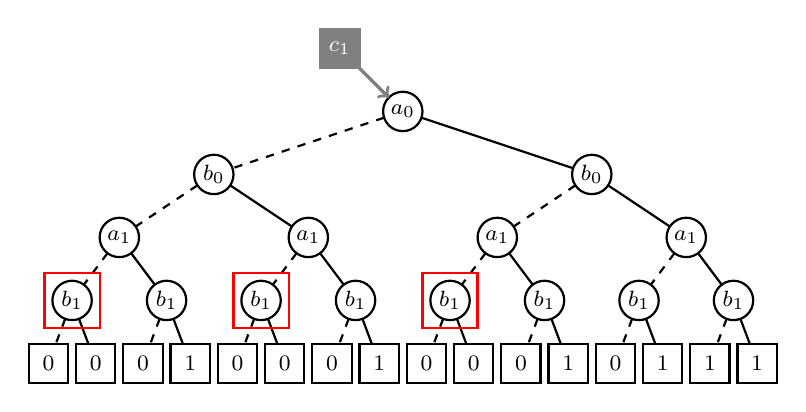
\begin{tikzpicture}
[every node/.style={draw=black,thick,minimum size=5mm,inner sep=0mm,outer sep=0mm,font=\footnotesize},
 var/.style={circle},
 val/.style={rectangle},
 ref/.style={rectangle,white,draw=gray,fill=gray},
 hl/.style={rectangle,draw=red,minimum size=7mm},
 thick]
\node[var] (a0)                                            {$a_0$};
\node[var] (b0A) [on grid,below  left=8mm and 24mm of a0]  {$b_0$};
\node[var] (b0B) [on grid,below right=8mm and 24mm of a0]  {$b_0$};
\node[var] (a1A) [on grid,below  left=8mm and 12mm of b0A] {$a_1$};
\node[var] (a1B) [on grid,below right=8mm and 12mm of b0A] {$a_1$};
\node[var] (a1C) [on grid,below  left=8mm and 12mm of b0B] {$a_1$};
\node[var] (a1D) [on grid,below right=8mm and 12mm of b0B] {$a_1$};
\node[var] (b1A) [on grid,below  left=8mm and  6mm of a1A] {$b_1$};
\node[var] (b1B) [on grid,below right=8mm and  6mm of a1A] {$b_1$};
\node[var] (b1C) [on grid,below  left=8mm and  6mm of a1B] {$b_1$};
\node[var] (b1D) [on grid,below right=8mm and  6mm of a1B] {$b_1$};
\node[var] (b1E) [on grid,below  left=8mm and  6mm of a1C] {$b_1$};
\node[var] (b1F) [on grid,below right=8mm and  6mm of a1C] {$b_1$};
\node[var] (b1G) [on grid,below  left=8mm and  6mm of a1D] {$b_1$};
\node[var] (b1H) [on grid,below right=8mm and  6mm of a1D] {$b_1$};
\node[val] (tA)  [on grid,below  left=8mm and  3mm of b1A] {0};
\node[val] (tB)  [on grid,below right=8mm and  3mm of b1A] {0};
\node[val] (tC)  [on grid,below  left=8mm and  3mm of b1B] {0};
\node[val] (tD)  [on grid,below right=8mm and  3mm of b1B] {1};
\node[val] (tE)  [on grid,below  left=8mm and  3mm of b1C] {0};
\node[val] (tF)  [on grid,below right=8mm and  3mm of b1C] {0};
\node[val] (tG)  [on grid,below  left=8mm and  3mm of b1D] {0};
\node[val] (tH)  [on grid,below right=8mm and  3mm of b1D] {1};
\node[val] (tI)  [on grid,below  left=8mm and  3mm of b1E] {0};
\node[val] (tJ)  [on grid,below right=8mm and  3mm of b1E] {0};
\node[val] (tK)  [on grid,below  left=8mm and  3mm of b1F] {0};
\node[val] (tL)  [on grid,below right=8mm and  3mm of b1F] {1};
\node[val] (tM)  [on grid,below  left=8mm and  3mm of b1G] {0};
\node[val] (tN)  [on grid,below right=8mm and  3mm of b1G] {1};
\node[val] (tO)  [on grid,below  left=8mm and  3mm of b1H] {1};
\node[val] (tP)  [on grid,below right=8mm and  3mm of b1H] {1};
\path[dashed] (a0)  edge (b0A);
\path         (a0)  edge (b0B);
\path[dashed] (b0A) edge (a1A);
\path         (b0A) edge (a1B);
\path[dashed] (b0B) edge (a1C);
\path         (b0B) edge (a1D);
\path[dashed] (a1A) edge (b1A);
\path         (a1A) edge (b1B);
\path[dashed] (a1B) edge (b1C);
\path         (a1B) edge (b1D);
\path[dashed] (a1C) edge (b1E);
\path         (a1C) edge (b1F);
\path[dashed] (a1D) edge (b1G);
\path         (a1D) edge (b1H);
\path[dashed] (b1A) edge (tA);
\path         (b1A) edge (tB);
\path[dashed] (b1B) edge (tC);
\path         (b1B) edge (tD);
\path[dashed] (b1C) edge (tE);
\path         (b1C) edge (tF);
\path[dashed] (b1D) edge (tG);
\path         (b1D) edge (tH);
\path[dashed] (b1E) edge (tI);
\path         (b1E) edge (tJ);
\path[dashed] (b1F) edge (tK);
\path         (b1F) edge (tL);
\path[dashed] (b1G) edge (tM);
\path         (b1G) edge (tN);
\path[dashed] (b1H) edge (tO);
\path         (b1H) edge (tP);

\node[ref] (Rc1) [on grid,above left=8mm and 8mm of a0] {$c_1$};
\path[->,gray,very thick] (Rc1) edge (a0);

\node[hl] [on grid,below=0mm of b1A] {};
\node[hl] [on grid,below=0mm of b1C] {};
\node[hl] [on grid,below=0mm of b1E] {};
\end{tikzpicture}

\end{figure}
\end{frame}

\begin{frame}
\begin{figure}
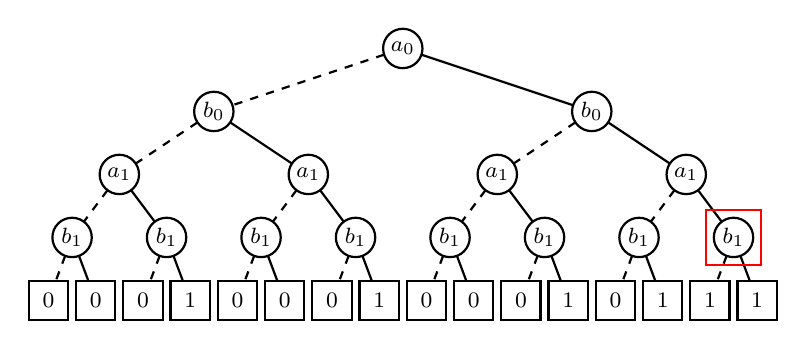
\begin{tikzpicture}
[every node/.style={draw=black,thick,minimum size=5mm,inner sep=0mm,outer sep=0mm,font=\footnotesize},
 var/.style={circle},
 val/.style={rectangle},
 hl/.style={rectangle,draw=red,minimum size=7mm},
 thick]
\node[var] (a0)                                            {$a_0$};
\node[var] (b0A) [on grid,below  left=8mm and 24mm of a0]  {$b_0$};
\node[var] (b0B) [on grid,below right=8mm and 24mm of a0]  {$b_0$};
\node[var] (a1A) [on grid,below  left=8mm and 12mm of b0A] {$a_1$};
\node[var] (a1B) [on grid,below right=8mm and 12mm of b0A] {$a_1$};
\node[var] (a1C) [on grid,below  left=8mm and 12mm of b0B] {$a_1$};
\node[var] (a1D) [on grid,below right=8mm and 12mm of b0B] {$a_1$};
\node[var] (b1A) [on grid,below  left=8mm and  6mm of a1A] {$b_1$};
\node[var] (b1B) [on grid,below right=8mm and  6mm of a1A] {$b_1$};
\node[var] (b1C) [on grid,below  left=8mm and  6mm of a1B] {$b_1$};
\node[var] (b1D) [on grid,below right=8mm and  6mm of a1B] {$b_1$};
\node[var] (b1E) [on grid,below  left=8mm and  6mm of a1C] {$b_1$};
\node[var] (b1F) [on grid,below right=8mm and  6mm of a1C] {$b_1$};
\node[var] (b1G) [on grid,below  left=8mm and  6mm of a1D] {$b_1$};
\node[var] (b1H) [on grid,below right=8mm and  6mm of a1D] {$b_1$};
\node[val] (tA)  [on grid,below  left=8mm and  3mm of b1A] {0};
\node[val] (tB)  [on grid,below right=8mm and  3mm of b1A] {0};
\node[val] (tC)  [on grid,below  left=8mm and  3mm of b1B] {0};
\node[val] (tD)  [on grid,below right=8mm and  3mm of b1B] {1};
\node[val] (tE)  [on grid,below  left=8mm and  3mm of b1C] {0};
\node[val] (tF)  [on grid,below right=8mm and  3mm of b1C] {0};
\node[val] (tG)  [on grid,below  left=8mm and  3mm of b1D] {0};
\node[val] (tH)  [on grid,below right=8mm and  3mm of b1D] {1};
\node[val] (tI)  [on grid,below  left=8mm and  3mm of b1E] {0};
\node[val] (tJ)  [on grid,below right=8mm and  3mm of b1E] {0};
\node[val] (tK)  [on grid,below  left=8mm and  3mm of b1F] {0};
\node[val] (tL)  [on grid,below right=8mm and  3mm of b1F] {1};
\node[val] (tM)  [on grid,below  left=8mm and  3mm of b1G] {0};
\node[val] (tN)  [on grid,below right=8mm and  3mm of b1G] {1};
\node[val] (tO)  [on grid,below  left=8mm and  3mm of b1H] {1};
\node[val] (tP)  [on grid,below right=8mm and  3mm of b1H] {1};
\path[dashed] (a0)  edge (b0A);
\path         (a0)  edge (b0B);
\path[dashed] (b0A) edge (a1A);
\path         (b0A) edge (a1B);
\path[dashed] (b0B) edge (a1C);
\path         (b0B) edge (a1D);
\path[dashed] (a1A) edge (b1A);
\path         (a1A) edge (b1B);
\path[dashed] (a1B) edge (b1C);
\path         (a1B) edge (b1D);
\path[dashed] (a1C) edge (b1E);
\path         (a1C) edge (b1F);
\path[dashed] (a1D) edge (b1G);
\path         (a1D) edge (b1H);
\path[dashed] (b1A) edge (tA);
\path         (b1A) edge (tB);
\path[dashed] (b1B) edge (tC);
\path         (b1B) edge (tD);
\path[dashed] (b1C) edge (tE);
\path         (b1C) edge (tF);
\path[dashed] (b1D) edge (tG);
\path         (b1D) edge (tH);
\path[dashed] (b1E) edge (tI);
\path         (b1E) edge (tJ);
\path[dashed] (b1F) edge (tK);
\path         (b1F) edge (tL);
\path[dashed] (b1G) edge (tM);
\path         (b1G) edge (tN);
\path[dashed] (b1H) edge (tO);
\path         (b1H) edge (tP);
\node[hl] [on grid,below=0mm of b1H] {};
\end{tikzpicture}

\end{figure}
\end{frame}

\begin{frame}
\begin{figure}
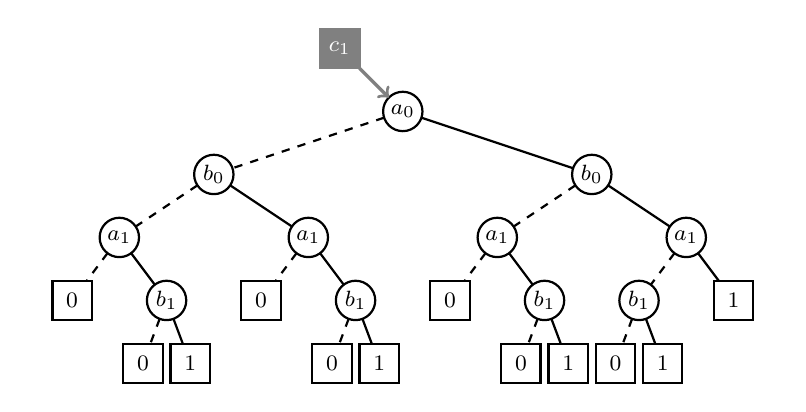
\begin{tikzpicture}
[every node/.style={draw=black,thick,minimum size=5mm,inner sep=0mm,outer sep=0mm,font=\footnotesize},
 var/.style={circle},
 val/.style={rectangle},
 ref/.style={rectangle,white,draw=gray,fill=gray},
 hl/.style={rectangle,draw=red,minimum size=7mm},
 thick]
\node[var] (a0)                                            {$a_0$};
\node[var] (b0A) [on grid,below  left=8mm and 24mm of a0]  {$b_0$};
\node[var] (b0B) [on grid,below right=8mm and 24mm of a0]  {$b_0$};
\node[var] (a1A) [on grid,below  left=8mm and 12mm of b0A] {$a_1$};
\node[var] (a1B) [on grid,below right=8mm and 12mm of b0A] {$a_1$};
\node[var] (a1C) [on grid,below  left=8mm and 12mm of b0B] {$a_1$};
\node[var] (a1D) [on grid,below right=8mm and 12mm of b0B] {$a_1$};
\node[val] (b1A) [on grid,below  left=8mm and  6mm of a1A] {0};
\node[var] (b1B) [on grid,below right=8mm and  6mm of a1A] {$b_1$};
\node[val] (b1C) [on grid,below  left=8mm and  6mm of a1B] {0};
\node[var] (b1D) [on grid,below right=8mm and  6mm of a1B] {$b_1$};
\node[val] (b1E) [on grid,below  left=8mm and  6mm of a1C] {0};
\node[var] (b1F) [on grid,below right=8mm and  6mm of a1C] {$b_1$};
\node[var] (b1G) [on grid,below  left=8mm and  6mm of a1D] {$b_1$};
\node[val] (b1H) [on grid,below right=8mm and  6mm of a1D] {1};
\node[val] (tC)  [on grid,below  left=8mm and  3mm of b1B] {0};
\node[val] (tD)  [on grid,below right=8mm and  3mm of b1B] {1};
\node[val] (tG)  [on grid,below  left=8mm and  3mm of b1D] {0};
\node[val] (tH)  [on grid,below right=8mm and  3mm of b1D] {1};
\node[val] (tK)  [on grid,below  left=8mm and  3mm of b1F] {0};
\node[val] (tL)  [on grid,below right=8mm and  3mm of b1F] {1};
\node[val] (tM)  [on grid,below  left=8mm and  3mm of b1G] {0};
\node[val] (tN)  [on grid,below right=8mm and  3mm of b1G] {1};
\path[dashed] (a0)  edge (b0A);
\path         (a0)  edge (b0B);
\path[dashed] (b0A) edge (a1A);
\path         (b0A) edge (a1B);
\path[dashed] (b0B) edge (a1C);
\path         (b0B) edge (a1D);
\path[dashed] (a1A) edge (b1A);
\path         (a1A) edge (b1B);
\path[dashed] (a1B) edge (b1C);
\path         (a1B) edge (b1D);
\path[dashed] (a1C) edge (b1E);
\path         (a1C) edge (b1F);
\path[dashed] (a1D) edge (b1G);
\path         (a1D) edge (b1H);
\path[dashed] (b1B) edge (tC);
\path         (b1B) edge (tD);
\path[dashed] (b1D) edge (tG);
\path         (b1D) edge (tH);
\path[dashed] (b1F) edge (tK);
\path         (b1F) edge (tL);
\path[dashed] (b1G) edge (tM);
\path         (b1G) edge (tN);

\node[ref] (Rc1) [on grid,above left=8mm and 8mm of a0] {$c_1$};
\path[->,gray,very thick] (Rc1) edge (a0);

% included on every picture to make sure a0 stays centered
\node[draw=white] (xA) [on grid,below  left=32mm and 45mm of a0] {};
\node[draw=white] (xb) [on grid,below right=32mm and 45mm of a0] {};
\end{tikzpicture}

\end{figure}
\end{frame}

\begin{frame}
\begin{figure}
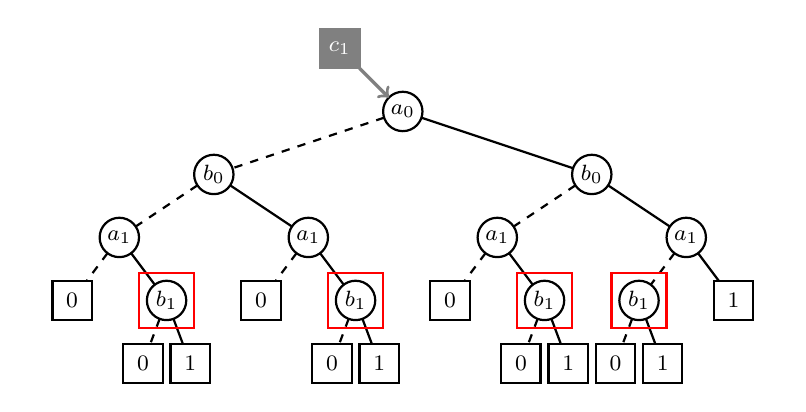
\begin{tikzpicture}
[every node/.style={draw=black,thick,minimum size=5mm,inner sep=0mm,outer sep=0mm,font=\footnotesize},
 var/.style={circle},
 val/.style={rectangle},
 ref/.style={rectangle,white,draw=gray,fill=gray},
 hl/.style={rectangle,draw=red,minimum size=7mm},
 thick]
\node[var] (a0)                                            {$a_0$};
\node[var] (b0A) [on grid,below  left=8mm and 24mm of a0]  {$b_0$};
\node[var] (b0B) [on grid,below right=8mm and 24mm of a0]  {$b_0$};
\node[var] (a1A) [on grid,below  left=8mm and 12mm of b0A] {$a_1$};
\node[var] (a1B) [on grid,below right=8mm and 12mm of b0A] {$a_1$};
\node[var] (a1C) [on grid,below  left=8mm and 12mm of b0B] {$a_1$};
\node[var] (a1D) [on grid,below right=8mm and 12mm of b0B] {$a_1$};
\node[val] (b1A) [on grid,below  left=8mm and  6mm of a1A] {0};
\node[var] (b1B) [on grid,below right=8mm and  6mm of a1A] {$b_1$};
\node[val] (b1C) [on grid,below  left=8mm and  6mm of a1B] {0};
\node[var] (b1D) [on grid,below right=8mm and  6mm of a1B] {$b_1$};
\node[val] (b1E) [on grid,below  left=8mm and  6mm of a1C] {0};
\node[var] (b1F) [on grid,below right=8mm and  6mm of a1C] {$b_1$};
\node[var] (b1G) [on grid,below  left=8mm and  6mm of a1D] {$b_1$};
\node[val] (b1H) [on grid,below right=8mm and  6mm of a1D] {1};
\node[val] (tC)  [on grid,below  left=8mm and  3mm of b1B] {0};
\node[val] (tD)  [on grid,below right=8mm and  3mm of b1B] {1};
\node[val] (tG)  [on grid,below  left=8mm and  3mm of b1D] {0};
\node[val] (tH)  [on grid,below right=8mm and  3mm of b1D] {1};
\node[val] (tK)  [on grid,below  left=8mm and  3mm of b1F] {0};
\node[val] (tL)  [on grid,below right=8mm and  3mm of b1F] {1};
\node[val] (tM)  [on grid,below  left=8mm and  3mm of b1G] {0};
\node[val] (tN)  [on grid,below right=8mm and  3mm of b1G] {1};
\path[dashed] (a0)  edge (b0A);
\path         (a0)  edge (b0B);
\path[dashed] (b0A) edge (a1A);
\path         (b0A) edge (a1B);
\path[dashed] (b0B) edge (a1C);
\path         (b0B) edge (a1D);
\path[dashed] (a1A) edge (b1A);
\path         (a1A) edge (b1B);
\path[dashed] (a1B) edge (b1C);
\path         (a1B) edge (b1D);
\path[dashed] (a1C) edge (b1E);
\path         (a1C) edge (b1F);
\path[dashed] (a1D) edge (b1G);
\path         (a1D) edge (b1H);
\path[dashed] (b1B) edge (tC);
\path         (b1B) edge (tD);
\path[dashed] (b1D) edge (tG);
\path         (b1D) edge (tH);
\path[dashed] (b1F) edge (tK);
\path         (b1F) edge (tL);
\path[dashed] (b1G) edge (tM);
\path         (b1G) edge (tN);

\node[ref] (Rc1) [on grid,above left=8mm and 8mm of a0] {$c_1$};
\path[->,gray,very thick] (Rc1) edge (a0);

\node[hl] [on grid,below=0mm of b1B] {};
\node[hl] [on grid,below=0mm of b1D] {};
\node[hl] [on grid,below=0mm of b1F] {};
\node[hl] [on grid,below=0mm of b1G] {};

% included on every picture to make sure a0 stays centered
\node[draw=white] (xA) [on grid,below  left=32mm and 45mm of a0] {};
\node[draw=white] (xb) [on grid,below right=32mm and 45mm of a0] {};
\end{tikzpicture}

\end{figure}
\end{frame}

\begin{frame}
\begin{figure}
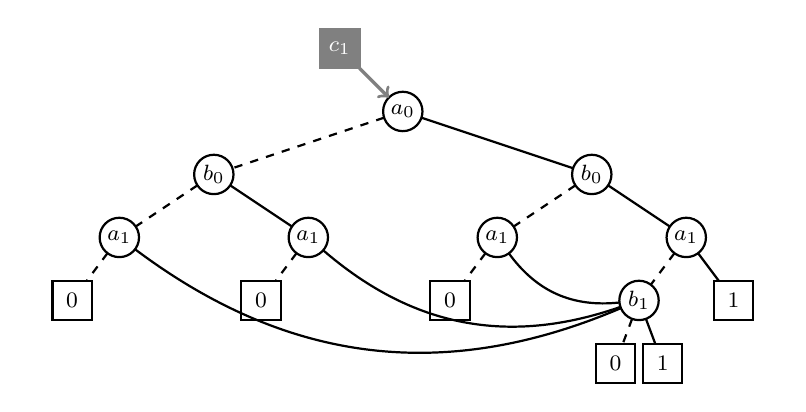
\begin{tikzpicture}
[every node/.style={draw=black,thick,minimum size=5mm,inner sep=0mm,outer sep=0mm,font=\footnotesize},
 var/.style={circle},
 val/.style={rectangle},
 ref/.style={rectangle,white,draw=gray,fill=gray},
 hl/.style={rectangle,draw=red,minimum size=7mm},
 thick]
\node[var] (a0)                                            {$a_0$};
\node[var] (b0A) [on grid,below  left=8mm and 24mm of a0]  {$b_0$};
\node[var] (b0B) [on grid,below right=8mm and 24mm of a0]  {$b_0$};
\node[var] (a1A) [on grid,below  left=8mm and 12mm of b0A] {$a_1$};
\node[var] (a1B) [on grid,below right=8mm and 12mm of b0A] {$a_1$};
\node[var] (a1C) [on grid,below  left=8mm and 12mm of b0B] {$a_1$};
\node[var] (a1D) [on grid,below right=8mm and 12mm of b0B] {$a_1$};
\node[val] (b1A) [on grid,below  left=8mm and  6mm of a1A] {0};
\node[val] (b1C) [on grid,below  left=8mm and  6mm of a1B] {0};
\node[val] (b1E) [on grid,below  left=8mm and  6mm of a1C] {0};
\node[var] (b1G) [on grid,below  left=8mm and  6mm of a1D] {$b_1$};
\node[val] (b1H) [on grid,below right=8mm and  6mm of a1D] {1};
\node[val] (tM)  [on grid,below  left=8mm and  3mm of b1G] {0};
\node[val] (tN)  [on grid,below right=8mm and  3mm of b1G] {1};
\path[dashed]     (a0)  edge (b0A);
\path             (a0)  edge (b0B);
\path[dashed]     (b0A) edge (a1A);
\path             (b0A) edge (a1B);
\path[dashed]     (b0B) edge (a1C);
\path             (b0B) edge (a1D);
\path[dashed]     (a1A) edge (b1A);
\path[bend right] (a1A) edge (b1G);
\path[dashed]     (a1B) edge (b1C);
\path[bend right] (a1B) edge (b1G);
\path[dashed]     (a1C) edge (b1E);
\path[bend right] (a1C) edge (b1G);
\path[dashed]     (a1D) edge (b1G);
\path             (a1D) edge (b1H);
\path[dashed]     (b1G) edge (tM);
\path             (b1G) edge (tN);

\node[ref] (Rc1) [on grid,above left=8mm and 8mm of a0] {$c_1$};
\path[->,gray,very thick] (Rc1) edge (a0);

% included on every picture to make sure a0 stays centered
\node[draw=white] (xA) [on grid,below  left=32mm and 45mm of a0] {};
\node[draw=white] (xb) [on grid,below right=32mm and 45mm of a0] {};
\end{tikzpicture}

\end{figure}
\end{frame}

\begin{frame}
\begin{figure}
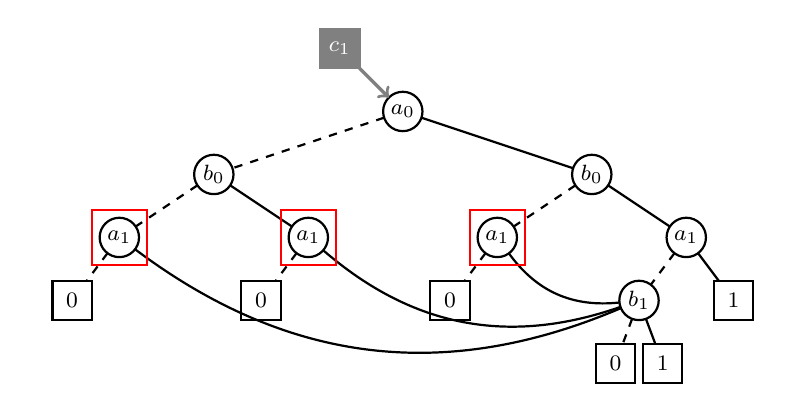
\begin{tikzpicture}
[every node/.style={draw=black,thick,minimum size=5mm,inner sep=0mm,outer sep=0mm,font=\footnotesize},
 var/.style={circle},
 val/.style={rectangle},
 ref/.style={rectangle,white,draw=gray,fill=gray},
 hl/.style={rectangle,draw=red,minimum size=7mm},
 thick]
\node[var] (a0)                                            {$a_0$};
\node[var] (b0A) [on grid,below  left=8mm and 24mm of a0]  {$b_0$};
\node[var] (b0B) [on grid,below right=8mm and 24mm of a0]  {$b_0$};
\node[var] (a1A) [on grid,below  left=8mm and 12mm of b0A] {$a_1$};
\node[var] (a1B) [on grid,below right=8mm and 12mm of b0A] {$a_1$};
\node[var] (a1C) [on grid,below  left=8mm and 12mm of b0B] {$a_1$};
\node[var] (a1D) [on grid,below right=8mm and 12mm of b0B] {$a_1$};
\node[val] (b1A) [on grid,below  left=8mm and  6mm of a1A] {0};
\node[val] (b1C) [on grid,below  left=8mm and  6mm of a1B] {0};
\node[val] (b1E) [on grid,below  left=8mm and  6mm of a1C] {0};
\node[var] (b1G) [on grid,below  left=8mm and  6mm of a1D] {$b_1$};
\node[val] (b1H) [on grid,below right=8mm and  6mm of a1D] {1};
\node[val] (tM)  [on grid,below  left=8mm and  3mm of b1G] {0};
\node[val] (tN)  [on grid,below right=8mm and  3mm of b1G] {1};
\path[dashed]     (a0)  edge (b0A);
\path             (a0)  edge (b0B);
\path[dashed]     (b0A) edge (a1A);
\path             (b0A) edge (a1B);
\path[dashed]     (b0B) edge (a1C);
\path             (b0B) edge (a1D);
\path[dashed]     (a1A) edge (b1A);
\path[bend right] (a1A) edge (b1G);
\path[dashed]     (a1B) edge (b1C);
\path[bend right] (a1B) edge (b1G);
\path[dashed]     (a1C) edge (b1E);
\path[bend right] (a1C) edge (b1G);
\path[dashed]     (a1D) edge (b1G);
\path             (a1D) edge (b1H);
\path[dashed]     (b1G) edge (tM);
\path             (b1G) edge (tN);

\node[ref] (Rc1) [on grid,above left=8mm and 8mm of a0] {$c_1$};
\path[->,gray,very thick] (Rc1) edge (a0);

\node[hl] [on grid,below=0mm of a1A] {};
\node[hl] [on grid,below=0mm of a1B] {};
\node[hl] [on grid,below=0mm of a1C] {};

% included on every picture to make sure a0 stays centered
\node[draw=white] (xA) [on grid,below  left=32mm and 45mm of a0] {};
\node[draw=white] (xb) [on grid,below right=32mm and 45mm of a0] {};
\end{tikzpicture}

\end{figure}
\end{frame}

\begin{frame}
\begin{figure}
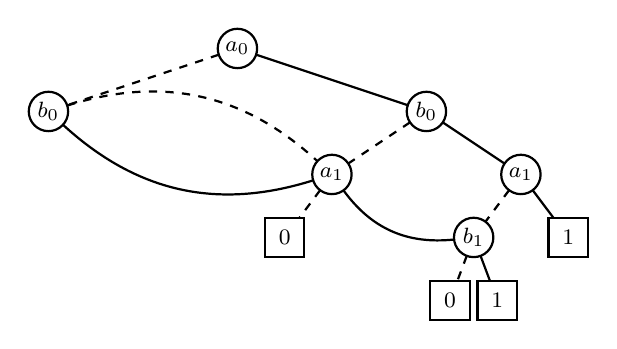
\begin{tikzpicture}
[every node/.style={draw=black,thick,minimum size=5mm,inner sep=0mm,outer sep=0mm,font=\footnotesize},
 var/.style={circle},
 val/.style={rectangle},
 thick]
\node[var] (a0)                                            {$a_0$};
\node[var] (b0A) [on grid,below  left=8mm and 24mm of a0]  {$b_0$};
\node[var] (b0B) [on grid,below right=8mm and 24mm of a0]  {$b_0$};
\node[var] (a1C) [on grid,below  left=8mm and 12mm of b0B] {$a_1$};
\node[var] (a1D) [on grid,below right=8mm and 12mm of b0B] {$a_1$};
\node[val] (b1E) [on grid,below  left=8mm and  6mm of a1C] {0};
\node[var] (b1G) [on grid,below  left=8mm and  6mm of a1D] {$b_1$};
\node[val] (b1H) [on grid,below right=8mm and  6mm of a1D] {1};
\node[val] (tM)  [on grid,below  left=8mm and  3mm of b1G] {0};
\node[val] (tN)  [on grid,below right=8mm and  3mm of b1G] {1};
\path[dashed]           (a0)  edge (b0A);
\path                   (a0)  edge (b0B);
\path[bend left,dashed] (b0A) edge (a1C);
\path[bend right]       (b0A) edge (a1C);
\path[dashed]           (b0B) edge (a1C);
\path                   (b0B) edge (a1D);
\path[dashed]           (a1C) edge (b1E);
\path[bend right]       (a1C) edge (b1G);
\path[dashed]           (a1D) edge (b1G);
\path                   (a1D) edge (b1H);
\path[dashed]           (b1G) edge (tM);
\path                   (b1G) edge (tN);
\end{tikzpicture}

\end{figure}
\end{frame}

\begin{frame}
\begin{figure}
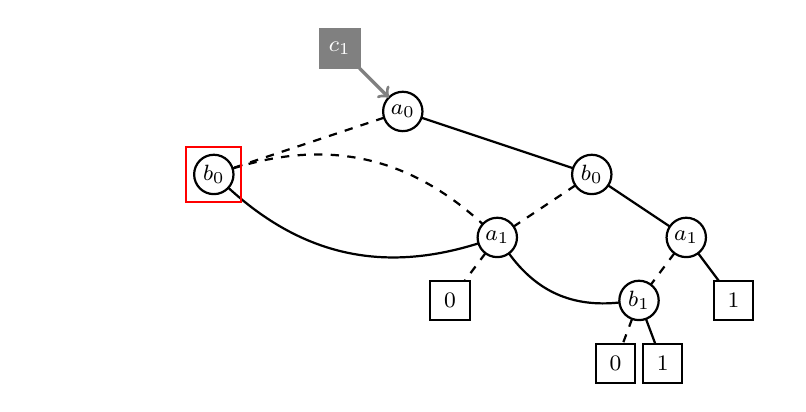
\begin{tikzpicture}
[every node/.style={draw=black,thick,minimum size=5mm,inner sep=0mm,outer sep=0mm,font=\footnotesize},
 var/.style={circle},
 val/.style={rectangle},
 ref/.style={rectangle,white,draw=gray,fill=gray},
 hl/.style={rectangle,draw=red,minimum size=7mm},
 thick]
\node[var] (a0)                                            {$a_0$};
\node[var] (b0A) [on grid,below  left=8mm and 24mm of a0]  {$b_0$};
\node[var] (b0B) [on grid,below right=8mm and 24mm of a0]  {$b_0$};
\node[var] (a1C) [on grid,below  left=8mm and 12mm of b0B] {$a_1$};
\node[var] (a1D) [on grid,below right=8mm and 12mm of b0B] {$a_1$};
\node[val] (b1E) [on grid,below  left=8mm and  6mm of a1C] {0};
\node[var] (b1G) [on grid,below  left=8mm and  6mm of a1D] {$b_1$};
\node[val] (b1H) [on grid,below right=8mm and  6mm of a1D] {1};
\node[val] (tM)  [on grid,below  left=8mm and  3mm of b1G] {0};
\node[val] (tN)  [on grid,below right=8mm and  3mm of b1G] {1};
\path[dashed]           (a0)  edge (b0A);
\path                   (a0)  edge (b0B);
\path[bend left,dashed] (b0A) edge (a1C);
\path[bend right]       (b0A) edge (a1C);
\path[dashed]           (b0B) edge (a1C);
\path                   (b0B) edge (a1D);
\path[dashed]           (a1C) edge (b1E);
\path[bend right]       (a1C) edge (b1G);
\path[dashed]           (a1D) edge (b1G);
\path                   (a1D) edge (b1H);
\path[dashed]           (b1G) edge (tM);
\path                   (b1G) edge (tN);

\node[ref] (Rc1) [on grid,above left=8mm and 8mm of a0] {$c_1$};
\path[->,gray,very thick] (Rc1) edge (a0);

\node[hl] [on grid,below=0mm of b0A] {};

% included on every picture to make sure a0 stays centered
\node[draw=white] (xA) [on grid,below  left=32mm and 45mm of a0] {};
\node[draw=white] (xb) [on grid,below right=32mm and 45mm of a0] {};
\end{tikzpicture}

\end{figure}
\end{frame}

\begin{frame}
\begin{figure}
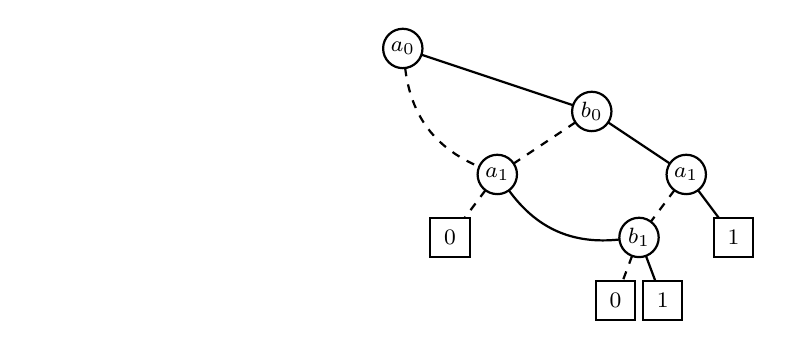
\begin{tikzpicture}
[every node/.style={draw=black,thick,minimum size=5mm,inner sep=0mm,outer sep=0mm,font=\footnotesize},
 var/.style={circle},
 val/.style={rectangle},
 hl/.style={rectangle,draw=red,minimum size=7mm},
 thick]
\node[var] (a0)                                            {$a_0$};
\node[var] (b0B) [on grid,below right=8mm and 24mm of a0]  {$b_0$};
\node[var] (a1C) [on grid,below  left=8mm and 12mm of b0B] {$a_1$};
\node[var] (a1D) [on grid,below right=8mm and 12mm of b0B] {$a_1$};
\node[val] (b1E) [on grid,below  left=8mm and  6mm of a1C] {0};
\node[var] (b1G) [on grid,below  left=8mm and  6mm of a1D] {$b_1$};
\node[val] (b1H) [on grid,below right=8mm and  6mm of a1D] {1};
\node[val] (tM)  [on grid,below  left=8mm and  3mm of b1G] {0};
\node[val] (tN)  [on grid,below right=8mm and  3mm of b1G] {1};
\path[bend right,dashed] (a0)  edge (a1C);
\path                    (a0)  edge (b0B);
\path[dashed]            (b0B) edge (a1C);
\path                    (b0B) edge (a1D);
\path[dashed]            (a1C) edge (b1E);
\path[bend right]        (a1C) edge (b1G);
\path[dashed]            (a1D) edge (b1G);
\path                    (a1D) edge (b1H);
\path[dashed]            (b1G) edge (tM);
\path                    (b1G) edge (tN);

% included on every picture to make sure a0 stays centered
\node[draw=white] (xA) [on grid,below  left=32mm and 45mm of a0] {};
\node[draw=white] (xb) [on grid,below right=32mm and 45mm of a0] {};
\end{tikzpicture}

\end{figure}
\end{frame}

\begin{frame}
\begin{figure}
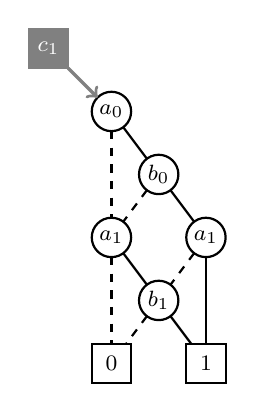
\begin{tikzpicture}
[every node/.style={draw=black,thick,minimum size=5mm,inner sep=0mm,outer sep=0mm,font=\footnotesize},
 var/.style={circle},
 val/.style={rectangle},
 ref/.style={rectangle,white,draw=gray,fill=gray},
 hl/.style={rectangle,draw=red,minimum size=7mm},
 thick]
\node[var] (a0)                                           {$a_0$};
\node[var] (b0B) [on grid,below right=8mm and 6mm of a0]  {$b_0$};
\node[var] (a1C) [on grid,below  left=8mm and 6mm of b0B] {$a_1$};
\node[var] (a1D) [on grid,below right=8mm and 6mm of b0B] {$a_1$};
\node[var] (b1G) [on grid,below  left=8mm and 6mm of a1D] {$b_1$};
\node[val] (tM)  [on grid,below  left=8mm and 6mm of b1G] {0};
\node[val] (tN)  [on grid,below right=8mm and 6mm of b1G] {1};
\path[dashed] (a0)  edge (a1C);
\path         (a0)  edge (b0B);
\path[dashed] (b0B) edge (a1C);
\path         (b0B) edge (a1D);
\path[dashed] (a1C) edge (tM);
\path         (a1C) edge (b1G);
\path[dashed] (a1D) edge (b1G);
\path         (a1D) edge (tN);
\path[dashed] (b1G) edge (tM);
\path         (b1G) edge (tN);

\node[ref] (Rc1) [on grid,above left=8mm and 8mm of a0] {$c_1$};
\path[->,gray,very thick] (Rc1) edge (a0);
\end{tikzpicture}

\end{figure}
\end{frame}

\begin{frame}
\begin{figure}
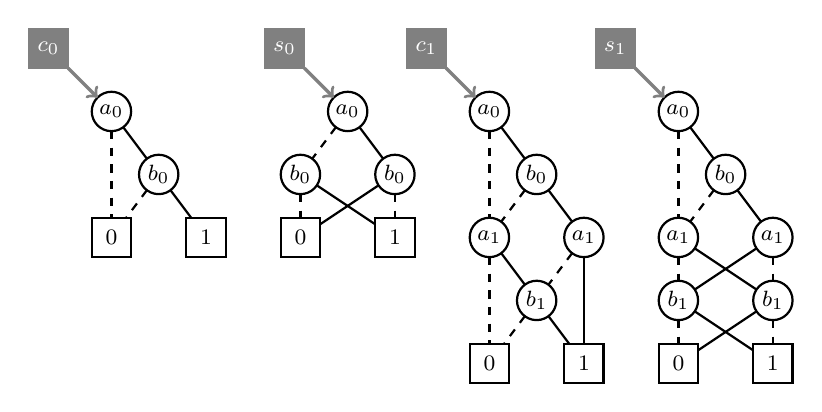
\begin{tikzpicture}
[every node/.style={draw=black,thick,minimum size=5mm,inner sep=0mm,outer sep=0mm,font=\footnotesize},
 var/.style={circle},
 val/.style={rectangle},
 ref/.style={rectangle,white,draw=gray,fill=gray},
 thick]

% c0
\node[var] (C0a0)                                           {$a_0$};
\node[var] (C0b0) [on grid,below right=8mm and 6mm of C0a0] {$b_0$};
\node[val] (C0t0) [on grid,below  left=8mm and 6mm of C0b0] {0};
\node[val] (C0t1) [on grid,below right=8mm and 6mm of C0b0] {1};
\path[dashed] (C0a0) edge (C0t0);
\path         (C0a0) edge (C0b0);
\path[dashed] (C0b0) edge (C0t0);
\path         (C0b0) edge (C0t1);

% s0
\node[var] (S0a0)  [on grid,right=30mm              of C0a0] {$a_0$};
\node[var] (S0b0A) [on grid,below  left=8mm and 6mm of S0a0] {$b_0$};
\node[var] (S0b0B) [on grid,below right=8mm and 6mm of S0a0] {$b_0$};
\node[val] (S0t0)  [on grid,below=8mm of S0b0A] {0};
\node[val] (S0t1)  [on grid,below=8mm of S0b0B] {1};
\path[dashed] (S0a0)  edge (S0b0A);
\path         (S0a0)  edge (S0b0B);
\path[dashed] (S0b0A) edge (S0t0);
\path         (S0b0A) edge (S0t1);
\path[dashed] (S0b0B) edge (S0t1);
\path         (S0b0B) edge (S0t0);

% c1
\node[var] (C1a0)  [on grid,right=18mm              of S0a0]  {$a_0$};
\node[var] (C1b0)  [on grid,below right=8mm and 6mm of C1a0]  {$b_0$};
\node[var] (C1a1A) [on grid,below  left=8mm and 6mm of C1b0]  {$a_1$};
\node[var] (C1a1B) [on grid,below right=8mm and 6mm of C1b0]  {$a_1$};
\node[var] (C1b1)  [on grid,below  left=8mm and 6mm of C1a1B] {$b_1$};
\node[val] (C1t0)  [on grid,below  left=8mm and 6mm of C1b1]  {0};
\node[val] (C1t1)  [on grid,below right=8mm and 6mm of C1b1]  {1};
\path[dashed] (C1a0)  edge (C1a1A);
\path         (C1a0)  edge (C1b0);
\path[dashed] (C1b0)  edge (C1a1A);
\path         (C1b0)  edge (C1a1B);
\path[dashed] (C1a1A) edge (C1t0);
\path         (C1a1A) edge (C1b1);
\path[dashed] (C1a1B) edge (C1b1);
\path         (C1a1B) edge (C1t1);
\path[dashed] (C1b1)  edge (C1t0);
\path         (C1b1)  edge (C1t1);

% s1
\node[var] (S1a0)  [on grid,right=24mm              of C1a0]  {$a_0$};
\node[var] (S1b0)  [on grid,below right=8mm and 6mm of S1a0]  {$b_0$};
\node[var] (S1a1A) [on grid,below  left=8mm and 6mm of S1b0]  {$a_1$};
\node[var] (S1a1B) [on grid,below right=8mm and 6mm of S1b0]  {$a_1$};
\node[var] (S1b1A) [on grid,below=8mm               of S1a1A] {$b_1$};
\node[var] (S1b1B) [on grid,below=8mm               of S1a1B] {$b_1$};
\node[val] (S1t0)  [on grid,below=8mm               of S1b1A] {0};
\node[val] (S1t1)  [on grid,below=8mm               of S1b1B] {1};
\path[dashed] (S1a0)  edge (S1a1A);
\path         (S1a0)  edge (S1b0);
\path[dashed] (S1b0)  edge (S1a1A);
\path         (S1b0)  edge (S1a1B);
\path[dashed] (S1a1A) edge (S1b1A);
\path         (S1a1A) edge (S1b1B);
\path[dashed] (S1a1B) edge (S1b1B);
\path         (S1a1B) edge (S1b1A);
\path[dashed] (S1b1A) edge (S1t0);
\path         (S1b1A) edge (S1t1);
\path[dashed] (S1b1B) edge (S1t1);
\path         (S1b1B) edge (S1t0);

\node[ref] (Rs0) [on grid,above left=8mm and 8mm of S0a0] {$s_0$};
\node[ref] (Rc0) [on grid,above left=8mm and 8mm of C0a0] {$c_0$};
\node[ref] (Rs1) [on grid,above left=8mm and 8mm of S1a0] {$s_1$};
\node[ref] (Rc1) [on grid,above left=8mm and 8mm of C1a0] {$c_1$};
\path[->,gray,very thick] (Rs0) edge (S0a0);
\path[->,gray,very thick] (Rc0) edge (C0a0);
\path[->,gray,very thick] (Rs1) edge (S1a0);
\path[->,gray,very thick] (Rc1) edge (C1a0);

\end{tikzpicture}

\end{figure}
\end{frame}

\begin{frame}
\begin{figure}
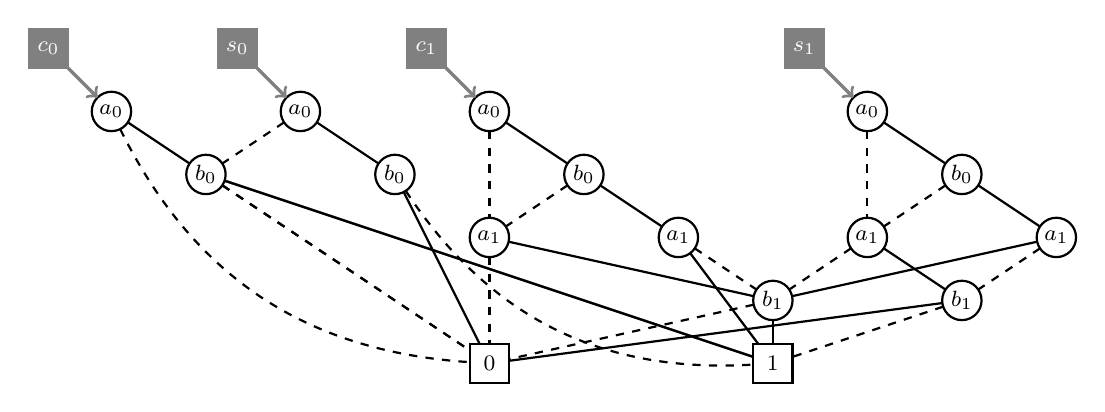
\begin{tikzpicture}
[every node/.style={draw=black,thick,minimum size=5mm,inner sep=0mm,outer sep=0mm,font=\footnotesize},
 var/.style={circle},
 val/.style={rectangle},
 ref/.style={rectangle,white,draw=gray,fill=gray},
 thick]

% c0
\node[var] (C0a0)  [on grid]                                   {$a_0$};
\node[var] (C0b0)  [on grid,below right=8mm and 12mm of C0a0]  {$b_0$};

% s0
\node[var] (S0a0)  [on grid,right=24mm of C0a0]                {$a_0$};
\node[var] (S0b0)  [on grid,below right=8mm and 12mm of S0a0]  {$b_0$};

% c1
\node[var] (C1a0)  [on grid,right=24mm of S0a0]                {$a_0$};
\node[var] (C1b0)  [on grid,below right=8mm and 12mm of C1a0]  {$b_0$};
\node[var] (C1a1A) [on grid,below  left=8mm and 12mm of C1b0]  {$a_1$};
\node[var] (C1a1B) [on grid,below right=8mm and 12mm of C1b0]  {$a_1$};

% s1
\node[var] (S1a0)  [on grid,right=48mm of C1a0]                {$a_0$};
\node[var] (S1b0)  [on grid,below right=8mm and 12mm of S1a0]  {$b_0$};
\node[var] (S1a1A) [on grid,below  left=8mm and 12mm of S1b0]  {$a_1$};
\node[var] (S1a1B) [on grid,below right=8mm and 12mm of S1b0]  {$a_1$};
\node[var] (S1b1A) [on grid,below  left=8mm and 12mm of S1a1A] {$b_1$};
\node[var] (S1b1B) [on grid,below right=8mm and 12mm of S1a1A] {$b_1$};

\node[val] (0)     [on grid,below=16mm of C1a1A]               {0};
\node[val] (1)     [on grid,below=8mm of S1b1A]                {1};

\path[dashed,bend right] (C0a0)  edge (0);
\path                    (C0a0)  edge (C0b0);
\path[dashed]            (C0b0)  edge (0);
\path                    (C0b0)  edge (1);

\path[dashed]            (S0a0)  edge (C0b0);
\path                    (S0a0)  edge (S0b0);
\path[dashed]            (C0b0)  edge (0);
\path                    (C0b0)  edge (1);
\path[dashed,bend right] (S0b0)  edge (1);
\path                    (S0b0)  edge (0);

\path[dashed]            (C1a0)  edge (C1a1A);
\path                    (C1a0)  edge (C1b0);
\path[dashed]            (C1a1A) edge (0);
\path                    (C1a1A) edge (S1b1A);
\path[dashed]            (C1a1B) edge (S1b1A);
\path                    (C1a1B) edge (1);
\path[dashed]            (C1b0)  edge (C1a1A);
\path                    (C1b0)  edge (C1a1B);

\path[dashed]            (S1a0)  edge (S1a1A);
\path                    (S1a0)  edge (S1b0);
\path[dashed]            (S1a1A) edge (S1b1A);
\path                    (S1a1A) edge (S1b1B);
\path[dashed]            (S1a1B) edge (S1b1B);
\path                    (S1a1B) edge (S1b1A);
\path[dashed]            (S1b0)  edge (S1a1A);
\path                    (S1b0)  edge (S1a1B);
\path[dashed]            (S1b1A) edge (0);
\path                    (S1b1A) edge (1);
\path[dashed]            (S1b1B) edge (1);
\path                    (S1b1B) edge (0);

\node[ref] (Rc0) [on grid,above left=8mm and 8mm of C0a0] {$c_0$};
\node[ref] (Rc1) [on grid,above left=8mm and 8mm of C1a0] {$c_1$};
\node[ref] (Rs0) [on grid,above left=8mm and 8mm of S0a0] {$s_0$};
\node[ref] (Rs1) [on grid,above left=8mm and 8mm of S1a0] {$s_1$};

\path[->,gray,very thick] (Rc0) edge (C0a0);
\path[->,gray,very thick] (Rc1) edge (C1a0);
\path[->,gray,very thick] (Rs0) edge (S0a0);
\path[->,gray,very thick] (Rs1) edge (S1a0);

\end{tikzpicture}

\end{figure}
\end{frame}

\begin{frame}
\end{frame}

\begin{frame}[shrink]
\begin{figure}
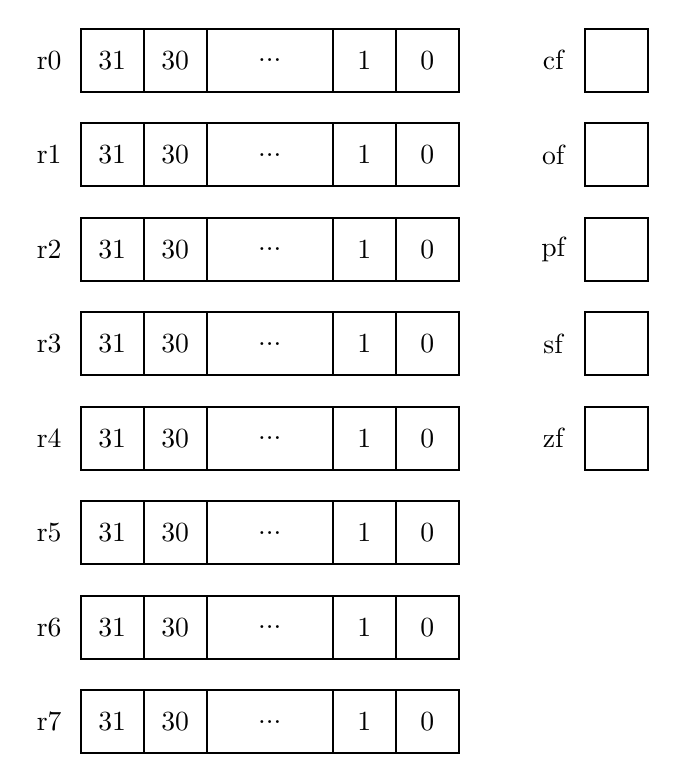
\begin{tikzpicture}[bit/.style={draw=black,minimum size=8mm,thick},etc/.style={draw=black,minimum width=16mm,minimum height=8mm,thick}]

\node      (r0)    [on grid]                     {r0};
\node[bit] (r0b31) [on grid,right= 8mm of r0]    {31};
\node[bit] (r0b30) [on grid,right= 8mm of r0b31] {30};
\node[etc] (r0etc) [on grid,right=12mm of r0b30] {...};
\node[bit] (r0b1)  [on grid,right=12mm of r0etc] {1};
\node[bit] (r0b0)  [on grid,right= 8mm of r0b1]  {0};

\node      (r1)    [on grid,below=12mm of r0]    {r1};
\node[bit] (r1b31) [on grid,right= 8mm of r1]    {31};
\node[bit] (r1b30) [on grid,right= 8mm of r1b31] {30};
\node[etc] (r1etc) [on grid,right=12mm of r1b30] {...};
\node[bit] (r1b1)  [on grid,right=12mm of r1etc] {1};
\node[bit] (r1b0)  [on grid,right= 8mm of r1b1]  {0};

\node      (r2)    [on grid,below=12mm of r1]    {r2};
\node[bit] (r2b31) [on grid,right= 8mm of r2]    {31};
\node[bit] (r2b30) [on grid,right= 8mm of r2b31] {30};
\node[etc] (r2etc) [on grid,right=12mm of r2b30] {...};
\node[bit] (r2b1)  [on grid,right=12mm of r2etc] {1};
\node[bit] (r2b0)  [on grid,right= 8mm of r2b1]  {0};

\node      (r3)    [on grid,below=12mm of r2]    {r3};
\node[bit] (r3b31) [on grid,right= 8mm of r3]    {31};
\node[bit] (r3b30) [on grid,right= 8mm of r3b31] {30};
\node[etc] (r3etc) [on grid,right=12mm of r3b30] {...};
\node[bit] (r3b1)  [on grid,right=12mm of r3etc] {1};
\node[bit] (r3b0)  [on grid,right= 8mm of r3b1]  {0};

\node      (r4)    [on grid,below=12mm of r3]    {r4};
\node[bit] (r4b31) [on grid,right= 8mm of r4]    {31};
\node[bit] (r4b30) [on grid,right= 8mm of r4b31] {30};
\node[etc] (r4etc) [on grid,right=12mm of r4b30] {...};
\node[bit] (r4b1)  [on grid,right=12mm of r4etc] {1};
\node[bit] (r4b0)  [on grid,right= 8mm of r4b1]  {0};

\node      (r5)    [on grid,below=12mm of r4]    {r5};
\node[bit] (r5b31) [on grid,right= 8mm of r5]    {31};
\node[bit] (r5b30) [on grid,right= 8mm of r5b31] {30};
\node[etc] (r5etc) [on grid,right=12mm of r5b30] {...};
\node[bit] (r5b1)  [on grid,right=12mm of r5etc] {1};
\node[bit] (r5b0)  [on grid,right= 8mm of r5b1]  {0};

\node      (r6)    [on grid,below=12mm of r5]    {r6};
\node[bit] (r6b31) [on grid,right= 8mm of r6]    {31};
\node[bit] (r6b30) [on grid,right= 8mm of r6b31] {30};
\node[etc] (r6etc) [on grid,right=12mm of r6b30] {...};
\node[bit] (r6b1)  [on grid,right=12mm of r6etc] {1};
\node[bit] (r6b0)  [on grid,right= 8mm of r6b1]  {0};

\node      (r7)    [on grid,below=12mm of r6]    {r7};
\node[bit] (r7b31) [on grid,right= 8mm of r7]    {31};
\node[bit] (r7b30) [on grid,right= 8mm of r7b31] {30};
\node[etc] (r7etc) [on grid,right=12mm of r7b30] {...};
\node[bit] (r7b1)  [on grid,right=12mm of r7etc] {1};
\node[bit] (r7b0)  [on grid,right= 8mm of r7b1]  {0};

\node      (cf)    [on grid,right=64mm of r0]    {cf};
\node[bit] (cfb)   [on grid,right= 8mm of cf]    {};

\node      (of)    [on grid,below=12mm of cf]    {of};
\node[bit] (ofb)   [on grid,right= 8mm of of]    {};

\node      (pf)    [on grid,below=12mm of of]    {pf};
\node[bit] (pfb)   [on grid,right= 8mm of pf]    {};

\node      (sf)    [on grid,below=12mm of pf]    {sf};
\node[bit] (sfb)   [on grid,right= 8mm of sf]    {};

\node      (zf)    [on grid,below=12mm of sf]    {zf};
\node[bit] (zfb)   [on grid,right= 8mm of zf]    {};

\end{tikzpicture}
\end{figure}
\end{frame}

\begin{frame}
\begin{table}
\tiny
\begin{tabular}{lllll}
flag control & data transfer & logic & addition/subtraction & multiplication \\
\hline
stc          & mov           & and   & add                  & imul           \\
clc          & cmovc         & or    & adc                  &                \\
cmc          & cmovo         & xor   & sub                  &                \\
             & cmovp         & not   & sbb                  &                \\
             & cmovs         &       & cmp                  &                \\
             & cmovz         &       & inc                  &                \\
             & cmovnc        &       & dec                  &                \\
             & cmovno        &       & neg                  &                \\
             & cmovnp        &       &                      &                \\
             & cmovns        &       &                      &                \\
             & cmovnz        &       &                      &                \\
             & cmova         &       &                      &                \\
             & cmovbe        &       &                      &                \\
             & cmovg         &       &                      &                \\
             & cmovge        &       &                      &                \\
             & cmovl         &       &                      &                \\
             & cmovle        &       &                      &                \\
\end{tabular}
\end{table}
\end{frame}

%\begin{frame}
%\begin{codebox}
%\Procname{$\proc{stc}()$}
%\zi $f_c \gets 1$
%\end{codebox}
%\end{frame}
%
%\begin{frame}
%\begin{codebox}
%\Procname{$\proc{mov}(a,b)$}
%\zi \For $i \gets 0$ \To $n-1$
%\zi \Do
%      $a_i \gets b_i$
%    \End
%\end{codebox}
%\end{frame}
%
%\begin{frame}
%\begin{codebox}
%\Procname{$\proc{cmov}(a,b)$}
%\zi $c \gets \id{condition}$
%\zi \For $i \gets 0$ \To $n-1$
%\zi \Do
%      $a_i \gets \NOT c \AND a_i \IOR c \AND b_i$
%    \End
%\end{codebox}
%\end{frame}
%
%\begin{frame}
%\begin{codebox}
%\Procname{$\proc{and}(a,b)$}
%\zi \For $i \gets 0$ \To $n-1$ \Do
%\zi   $a_i \gets a_i \AND b_i$ \End
%\zi $f_c \gets 0$
%\zi $f_o \gets 0$
%\zi $f_p \gets \NOT(a_0 \XOR a_1 \XOR ... \XOR a_7)$
%\zi $f_s \gets a_{n-1}$
%\zi $f_z \gets \NOT(a_0 \IOR a_1 \IOR ... \IOR a_{n-1})$
%\end{codebox}
%\end{frame}
%
%\begin{frame}
%\begin{codebox}
%\Procname{$\proc{add}(a,b)$}
%\zi $c_0 \gets a_0 \AND b_0$
%\zi $a_0 \gets a_0 \XOR b_0$
%\zi \For $i \gets 1$ \To $n-1$ \Do
%\zi   $c_i \gets a_i \AND b_i \IOR a_i \AND c_{i-1} \IOR b_i \AND c_{i-1}$
%\zi   $a_i \gets a_i \XOR b_i \XOR c_{i-1}$ \End
%\zi $f_c \gets c_{n-1}$
%\zi $f_o \gets c_{n-1} \XOR c_{n-2}$
%\zi $f_p \gets \NOT(a_0 \XOR a_1 \XOR ... \XOR a_7)$
%\zi $f_s \gets a_{n-1}$
%\zi $f_z \gets \NOT(a_0 \IOR a_1 \IOR ... \IOR a_{n-1})$
%\end{codebox}
%\end{frame}
%
%\begin{frame}
%\begin{codebox}
%\Procname{$\proc{imul}(a,b)$}
%\zi \For $j \gets 0 \To n-1$ \Do
%\zi   $x \gets a_{0} \AND b_{j}$
%\zi   $c_{j} \gets p_{j} \AND x$
%\zi   $p_{j} \gets p_{j} \XOR x$
%\zi   \For $i \gets j+1 \To 2n-1$ \Do
%\zi     $x \gets a_{i-j} \AND b_{j}$
%\zi     $c_{i} \gets p_{i} \AND x \IOR p_{i} \AND c_{i-1} \IOR x \AND c_{i-1}$
%\zi     $p_{i} \gets p_{i} \XOR x \XOR c_{i-1}$ \End \End
%\zi \For $i \gets 0 \To n-1$ \Do
%\zi   $a_{i} \gets p_{i}$ \End
%\zi $f_c \gets f_o \gets p_{n} \IOR p_{n+1} \IOR ... \IOR p_{2n-1}$
%\end{codebox}
%\end{frame}
%
%\begin{frame}
%\begin{codebox}
%\Procname{$\proc{imul}(a,b)$}
%\zi \For $j \gets 0 \To n-1$ \Do
%\zi   $x \gets a_{0} \AND b_{j}$
%\zi   $c_{j} \gets p_{j} \AND x$
%\zi   $p_{j} \gets p_{j} \XOR x$
%\zi   \For $i \gets j+1 \To n-1$ \Do
%\zi     $x \gets a_{i-j} \AND b_{j}$
%\zi     $c_{i} \gets p_{i} \AND x \IOR p_{i} \AND c_{i-1} \IOR x \AND c_{i-1}$
%\zi     $p_{i} \gets p_{i} \XOR x \XOR c_{i-1}$ \End
%\zi   \For $i \gets n \To 2n-1$ \Do
%\zi     $o \gets o \IOR a_{i-j} \AND b_{j}$ \End
%\zi   $o \gets o \IOR c_{n-1}$ \End
%\zi \For $i \gets 0 \To n-1$ \Do
%\zi   $a_{i} \gets p_{i}$ \End
%\zi $f_c \gets f_o \gets o$
%\end{codebox}
%\end{frame}

\begin{frame}
\end{frame}

%\begin{frame}
%\begin{codebox}
%\Procname{$\proc{sign}(a)$}
%\zi \If $a > 0$ \Do
%\zi   \Return $1$ \End
%\zi \If $a < 0$ \Do
%\zi   \Return $-1$ \End
%\zi \Return $0$
%\end{codebox}
%\end{frame}

\begin{frame}
\begin{table}
\tiny
\begin{tabular}{l|rrr}
length & & & \\
\hline
1 &         3 &   0 &   0 \\
2 &       155 &   0 &   0 \\
3 &     11849 &   0 &   0 \\
4 &   1082001 &   2 &   1 \\
5 & 121268867 & 326 & 209 \\
\end{tabular}
\end{table}
\end{frame}

%\begin{frame}
%\begin{center}
%add r0,r0; sbb r1,r1; sub r1,r0; adc r1,r0; \\
%add r0,r0; sbb r1,r1; neg r0; adc r1,r1;
%\end{center}
%\end{frame}
%
%\begin{frame}
%\begin{table}
%\tiny
%\begin{tabular}{l|lll}
%& r0 $>$ 0
%& r0 $<$ 0
%& r0 $=$ 0 \\
%\hline
%add r0,r0
%& \uncover<2->{r0 $\gets X$, cf $\gets 0$}
%& \uncover<3->{r0 $\gets Y$, cf $\gets 1$}
%& \uncover<4->{r0 $\gets 0$, cf $\gets 0$} \\
%sbb r1,r1
%& \uncover<2->{r1 $\gets 0$}
%& \uncover<3->{r1 $\gets -1$}
%& \uncover<4->{r1 $\gets 0$} \\
%sub r1,r0
%& \uncover<2->{r1 $\gets -X$, cf $\gets 1$}
%& \uncover<3->{r1 $\gets -1-Y$, cf $\gets 0$}
%& \uncover<4->{r1 $\gets 0$, cf $\gets 0$} \\
%adc r1,r0
%& \uncover<2->{r1 $\gets 1$}
%& \uncover<3->{r1 $\gets -1$}
%& \uncover<4->{r1 $\gets 0$} \\
%\end{tabular}
%\end{table}
%\end{frame}
%
%\begin{frame}
%\begin{table}
%\tiny
%\begin{tabular}{l|l}
%add r0,r0
%& \uncover<2->{r0 $\gets 0$, cf $\gets 1$} \\
%sbb r1,r1
%& \uncover<2->{r1 $\gets -1$} \\
%neg r0
%& \uncover<2->{r0 $\gets 0$, cf $\gets 0$} \\
%adc r1,r1
%& \uncover<2->{r1 $\gets -2$} \\
%\end{tabular}
%\end{table}
%\end{frame}

\begin{frame}
\end{frame}

\begin{frame}
\uncover<1->
{
\begin{table}
\tiny
\setlength{\tabcolsep}{1mm}
\begin{tabular}{l|l}
$P_0$ & mov r1,r0; \\
$P_1$ & xor r1,r1; and r1,r0; \\
$P_2$ & sub r1,r1; and r1,r0; \\
$P_3$ & xor r1,r1; add r1,r0; \\
$P_4$ & sub r1,r1; add r1,r0; \\
$P_5$ & add r0,r0; sbb r1,r1; inc r1; \\
$P_6$ & add r0,r0; sbb r1,r1; sub r1,r0; adc r1,r0; \\
$P_7$ & add r0,r0; sbb r1,r1; neg r0; adc r1,r1; \\
$P_8$ & xor r1,r1; xor r2,r2; xor r3,r3; inc r2; dec r3; cmp r1,r0; cmovl r1,r2; cmovg r1,r3; \\
\end{tabular}
\end{table}
}
\uncover<2->
{
\begin{table}
\tiny
\setlength{\tabcolsep}{1mm}
\begin{tabular}{*{9}{c}}
$P_0$    & $P_1$    & $P_2$    & $P_3$    & $P_4$    & $P_5$    & $P_6$    & $P_7$    & $P_8$    \\
\hline
0.119 ms & 0.175 ms & 0.284 ms & 0.281 ms & 0.389 ms & 0.447 ms & 0.966 ms & 0.679 ms & 0.673 ms \\
\end{tabular}
\end{table}
}
\uncover<3->
{
\begin{table}
\tiny
\setlength{\tabcolsep}{1mm}
\begin{tabular}{l|*{9}{c}}
      & $P_0$    & $P_1$    & $P_2$    & $P_3$    & $P_4$    & $P_5$    & $P_6$    & $P_7$    & $P_8$    \\
\hline
$P_0$ & 0.116 ms & 0.176 ms & 0.284 ms & 0.281 ms & 0.389 ms & 0.447 ms & 0.965 ms & 0.679 ms & 0.670 ms \\
$P_1$ &          & 0.235 ms & 0.343 ms & 0.340 ms & 0.449 ms & 0.507 ms & 1.025 ms & 0.757 ms & 0.729 ms \\
$P_2$ &          &          & 0.468 ms & 0.449 ms & 0.553 ms & 0.613 ms & 1.131 ms & 0.845 ms & 0.837 ms \\
$P_3$ &          &          &          & 0.422 ms & 0.529 ms & 0.592 ms & 1.107 ms & 0.821 ms & 0.834 ms \\
$P_4$ &          &          &          &          & 0.636 ms & 0.698 ms & 1.212 ms & 0.927 ms & 0.941 ms \\
$P_5$ &          &          &          &          &          & 0.752 ms & 1.270 ms & 0.984 ms & 1.001 ms \\
$P_6$ &          &          &          &          &          &          & 1.781 ms & 1.535 ms & 1.530 ms \\
$P_7$ &          &          &          &          &          &          &          & 1.171 ms & 1.224 ms \\
$P_8$ &          &          &          &          &          &          &          &          & 1.155 ms \\
\end{tabular}
\end{table}
}
\end{frame}

\begin{frame}
\end{frame}

\begin{frame}[shrink]
\begin{figure}
\include{performance_mul2}
\end{figure}
\end{frame}

\begin{frame}
\end{frame}

\end{document}
